\section{Context}
\label{sec:context}

This section presents definitions and background information necessary for a
full understanding of the problem.


\subsection{\Flaky Tests}
\label{sec:sec:flaky_tests}

A test consists of a set of inputs and a corresponding expected output, over
some subject under test. In a perfect world, a test always produces the expected
output provided the subject's behaviour is fixed. In reality, environmental and
chance factors can affect the actual output. We can model the expected output
probabilistically.

\begin{quote}
	A \flaky test is one known to fail with low probability.
\end{quote}

\begin{defn}[\Flaky Test]
\label{def:flaky_test}

Let $\vec{I}$ be the lifting of all inputs, including coin flips and
environmental interactions, into a single input vector. $\vec{O}$ is the
corresponding desired output. Given a subject under test $f: \vec{I} \rightarrow
\vec{O}$, a test case is $(\vec{i},\vec{o})$. A \emph{\flaky test case} is one
where
%
\begin{align*}
  p(f(\vec{i}) \ne \vec{o}) = \epsilon
\end{align*}
%
for non-negligible probability $\epsilon \in (0..\alpha]$.

\end{defn}

Flaky tests fail rarely.  What is {\lq}rare{\rq} depends on the problem and the
cost of the test.  If a test fails frequently enough, it can be converted into a
standard failing test by repeatedly running the test, subject to the cost of
that test.  The parameter $\alpha$ represents this threshold between
reproducible via repetition and not.  The exact probability $\epsilon$ must be
non-negligible so that repeated trials are likely to trigger the failure.  In
practice, this constraint is easily met, since it is hard to imagine that a
negligible $\epsilon$ matters.  Combined with our budget $B$
(\autoref{sec:sec:budget}), we can determine what values of $\epsilon$ we can
afford to detect.

Figure~\ref{fig:flakiness} depicts \flaky tests in terms of probability of
failure.

\begin{figure}[h]
\begin{center}
	% See: http://www.texample.net/tikz/examples/line-plot-example/
	\begin{tikzpicture}[thick, framed, x=6.5cm, y=1.6cm]
		% Title
		\draw (0.5, 1) node[above] {$\textsc{\flaky Test}$};

		% Axis
		\draw (0,0) -- coordinate (x axis mid) (1,0);
	    \draw (0,0) -- coordinate (y axis mid) (0,1);

	    % Axis Labels
	    \node (padding) [below] at (0.4, 0) {};
		\node[below of = padding] at (x axis mid) {Probability of Failure};

	    % Ticks
	    \foreach \x in {0, 1}
	    	\draw (\x, 1pt) -- (\x, -3pt) node[anchor=north] {\x};

		% \flaky test range
	    \draw[<-] (0, 0.5) -- (0.4, 0.5); % Draw horizontal line
	    \draw (0.4, 0.42) -- (0.4, 0.58); % Draw right vertical tab

	    % Flakiness label
	    \node [above] at (0.2, 0.5) {$Flaky$};

	    % Alpha label
	    \node [right] at (0.4, 0.5) {$(\boldsymbol{\alpha})$};
	\end{tikzpicture}
\end{center}
\caption{}
\label{fig:flakiness}
\end{figure}


\subsection{Automated Testing}
\label{sec:sec:automated_testing}

Automated testing has been adopted by developers globally, from those working in
start ups to those in major corporations. As the number of environments
deployments are expected to run in increases, testing all possible variants
quickly becomes unworkable. It is impractical to manually test an application
across hundreds of devices every time it is modified. Automated tests serve a
simple purpose --- ensure the software under test behaves as expected in the
supported set of environments. A good test suite achieves this by exercising
discrete chunks of the program's code to ensure it behaves in some expected way.
At a high level, each test can be broken into three steps - arrangement, action
and assertion.

Anecdotally, the higher-level the behaviour being tested, the more likely a test
is to fail due to inputs unaccounted for. Tests that exercise seemingly valid
code can fail unexpectedly and unpredictably. Developers working with such tests
face a dilemma --- {\lq}suppress{\rq} the tests until they are fixed, or
acknowledge them but keep them active, potentially randomly breaking the build
from time to time until they are fixed. Since the tests exercise behaviour which
is needed (and indeed, works as intended), both solutions are workarounds until
the tests can be resolved. A set of tests displaying seemingly random failure
can devalue an entire suite, so it is of utmost importance that developers fix
such issues as they arise. The test suite is not a user-facing feature and can
quickly become a cost rather than a benefit.

In our experience, within the context of real software development projects
developers quickly become frustrated when dealing with \flaky tests and begin to
rely on instinct in order to stay productive. In other words, they lose
confidence in the test suite. It is essential to maintain a reliable test suite
for it to remain a beneficial part of a team's workflow.


\subsection{Why Not {\lq}Non-Deterministic{\rq}?}

Nondeterministic has three possible meanings depending on the context. In
existing literature, practitioners tend to use non-deterministic in the Physics
sense --- \ie, probabalistic. Given that nondeterministic has different meanings
in Computer Science and Statistics/Probability, it is better to avoid confusion
and choose a suitable term: \flaky.


\subsection{Fixing \Flaky Tests the Manual Way}

Sometimes, it is not possible to fix a \flaky test from the information output
by the testrunner alone. Typically, the information includes logs, an assertion
failure message and/or a stack trace. Applications with a user interface may
also provide a number of screenshots. Often, a developer will have to manually
gather information to build up an understanding of the intended flow versus the
actual flow on failing runs. For \flaky tests with a low failure rate, this can
be a painstaking and time-consuming process, if not completely ineffective.
Indeed, if the \flaky test is a timing based issue, attaching a debugger may
cause the test to pass indefinitely due to the observer effect.

\subsubsection{Common Causes of Flakiness}

First, let us consider some common causes of flakiness:
\begin{itemize}
	\item Timeouts --- issues can occur when {\lq}driving{\rq} the application
	from the outside. Often, callbacks for actions are not available, so a test
	may be forced to wait on, for example, the presence of some element in the UI.
	If the wait time expires before the element is detected, the test will fail.
	\item Memory usage --- it is not uncommon for a constrained process to run out
	of memory. Again, this could be caused by operating system priorities
	unrelated to the test itself. It's obvious \textit{when} this has happened,
	but not \textit{why}.
	\item External services --- if a third party service falls over during a test
	run that depends on it, tests may fail.
	\item Left-over state --- static state can affect the execution of a test. If
	it is not cleaned up and reset, it can cause strange behaviour. This includes
	things like external databases, configuration files \etc.
\end{itemize}

Each developer familiar with these issues may employ techniques and patterns to
avoid them. However, while bug rates can be reduced, they are unlikely to ever
reach zero.

\Flaky tests are often split out into a seperate suite (a practice is known as
{\lq}quarantining{\rq}), so that developers may continue to receive the benefits
of a fast feedback cycle from the rest of the tests. This appears to be a
reasonable approach, but it is not a long term solution. Even if the tests are
fixed and moved from quarantine regularly, the benefits of the supressed tests
are completely lost once they are removed from the main test suite.

\subsubsection{Identification}

First, \flaky tests must be identified. How does a developer know if a failure
was genuine (\ie, failed due to a change in behaviour it was designed to test)
or unexpected?

Manual inspection of the related changeset and failure stacktrace is often
sufficient. A change in an area of the application (seemingly) entirely
unrelated to the observed test failure may indicate that the failure was indeed
unrelated and hence, the test \flaky. But, it is imprudent to operate on this
assumption alone. The test will then need to be re-run (either as part of the
suite on CI, or in isolation by the investigating developer locally). If the
test continues to fail, the change was clearly related. If not, the test is
\flaky.

The problem with this approach is that humans have limited memory. If the \flaky
test is not fixed as soon as it is identified (or moved to a quarantine), the
test can continue to cause problems further down the line. In fact, it can be
useful to examine test failure over time --- trends in failure may stand out.

A couple of projects have tackled this preliminary step of \flaky test
identification; namely, the Chromium Flakiness Dashboard
\cite{flakinessDashboard} and various Jenkins plugins. These tools typically run
as a continuous integration step. Some simply attach a value to each test
representing its likelihood of failure during any given test run. Others also
expose statistics such as \emph{stability($N$)} (the test's chance of failure
across the previous $N$ runs), successful runs since last failure and first
known failure. The Chromium Flakliness Dashboard includes a graphical matrix
view for visual detection of trends, displaying tests and their binary results
over time.

\begin{figure}[H]

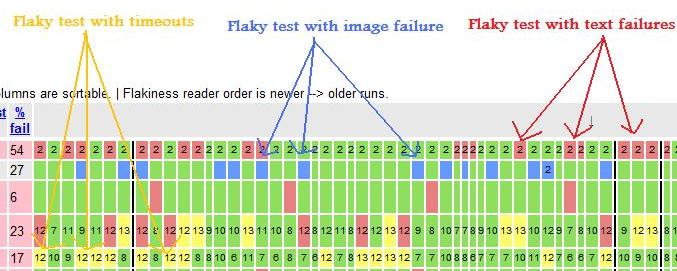
\includegraphics[width=\linewidth]{Images/chromium_flaky_dashboard}

\caption{The Chromium Flakiness Dashboard \cite{flakinessDashboard}}
\label{fig:chromium_dashboard}
\end{figure}

\subsubsection{Prioritisation}

With a host of known \flaky tests, either in quarantine or in the main test
suite, how does a developer decide which tests to fix first? There are several
obvious factors which may affect prioritisation, including:
\begin{itemize}
	\item Failure type --- multiple \flaky tests exhibiting similar problems may
	be tackled as a group. Certain failure types may be considered more critical
	than others.
	\item Age --- a \flaky test that has been known to be \flaky for a long period
	may be prioritised over more recent additions, or vice versa.
\end{itemize}

In the end, it is up to the development team to prioritise the \flaky tests, if
at all. With this in mind, the most useful thing we could do is expose
information to aid the decision making process. Providing the ability to group
and sort \flaky tests by the attributes listed above would no doubt be valuable.
In fact, this was an initial goal of the project, but it was eventually
sidelined in order to focus on the resolution phase.

\subsubsection{Resolution}

A common approach when fixing any bug (not just a \flaky test) is to step
through the code manually with the assistance of a debugger. By examining
execution flow and program state over one or more runs, a developer can often
pinpoint the cause or a related area of code. Debugging a \flaky acceptance test
in this way is often tedious, fruitless and time-consuming, especially if the
failure rate is low. Since an acceptance test must compile and run the entire
application, average run times can be extremely lengthy. If the test must
constantly be re-run in order to see it fail, this time quickly adds up. What's
more, attaching a debugger can affect the execution of the test, potentially
perturbing its behaviour.

An experienced developer may simply inspect the test in question to determine
the cause. The success of this method likely depends on the complexity and
familiarity of the bug.
